% To begin the document, load the 'knac' document class, which is a
% modified version of the AASTeX class.  Documentation for that
% package is available at http://aas.org/aastex/aastex-documentation.
%
% In your document, you can use almost any of the new LaTeX commands
% defined by the AASTeX package (e.g. \deluxetable, \ion, \lesssim,
% \sun, \arcmin, \micron, \citep, \bibitem, \apj, etc.  The main
% exceptions are AASTeX commands that are specific to publishing a
% journal article, e.g.  \received, \revised, \accepted, \slugcomment,
% \keywords, etc.  But almost any text-markup command should be OK.
% AASTex is the template for submission to the Journals run by the American 
% Astronomical Society (AAS). For Documentation on AASTex see: 
% https://journals.aas.org/aastex-package-for-manuscript-preparation/
% A general guide to the LateX markup language can be found here: 
% http://www.astrobetter.com/wiki/LaTeX 
% Overleaf.com is a popular online LaTeX Editor. 
% It has a guide here: https://www.overleaf.com/learn

\documentclass{knac}

% This next line is only necessary to get a live hyperlink in the
% output document:
\usepackage{hyperref}
\pagenumbering{gobble}  %Removes page numbers - do not remove this line!

%  If you want to define shortcuts for commonly-typed commands you'll
%  use, you can do so here - for example, here is a command to make it
%  easier to refer to H alpha emission (using 'math mode', denoted by
%  the dollar signs, to generate the Greek letter alpha). 

\newcommand{\ha}{H$\alpha$}


\begin{document}
% Give the title of the paper here. 
\title{How to Typeset a Paper for the KNAC Student Symposium Proceedings}

% Don't use the AASTeX-style commands \affil, \email, etc. for
% specifying various parts of the author or advisor information here -
% just give the author(s) and affiliation(s) just as you would like
% them to appear in the document:

\author{Student Author, Example College}

% If there are multiple advisors, use \advisors instead. 
\advisor{Helpful Advisor, Example College}


\begin{abstract}

  This document serves both as an example of how a symposium
  proceedings paper will appear, and as a guide to the procedure
  necessary to produce the paper in the proper format. Several key
  concepts are outlined, including how to cite references, examples of
  how to include figures and tables, and where to get help when you
  have questions.  To get the most out of this, you should read
  through the PDF output document produced, but also look at the
  source file (with the .tex extension), where the comments will give
  you additional information about how to produce the output you see
  here. 

\end{abstract}

%If you are only submitting an abstract, remove all of the text between here and the \end{document} command.

% After this comes your document.  You can use section headings with
% the \section command.  (And also \subsection if you wish.) 

\section{Introduction}

This is where the introductory text of the paper would go.  For
example, we can cite references in the text by using the \verb|\citep|
and \verb|\citet| commands, to cite the work of, for example,
\citet{Bary2002}, and others \citep{Kwitter2013, Willman2012}.  For
including references in the final reference list, you can get
Latex-formatted references directly from NASA ADS
(\url{http://www.adsabs.harvard.edu/abstract_service.html}) - after
finding the reference you want, click on ``Preferred format for this
abstract'' and you will get a \verb|\bibitem| record in \LaTeX\ format
that can be pasted into the references section of your document, and
referred to in the paper by a shorthand tag that you create; see the
source file of this document to see how it works.

% Below is code for an example figure, illustrating how to include the
% graphics file.  Notice that it's not necessary to number the figures
% or tables explicitly - Latex takes care of that, numbering them in
% the order they appear. 

% The file included in this example is a PDF file. This is the default for Macs and 
% Overleaf (overleaf.com) - which is an online Latex editor. 

% If you are playing around with this file to learn about Latex, try
% changing the filename below in the \includegraphics command to
% reference one of your own figures. 

\begin{figure}[bht]
% Make sure the figure is centered:
\centering
% Include the file - notice that we can rotate it and scale it as
% needed: 
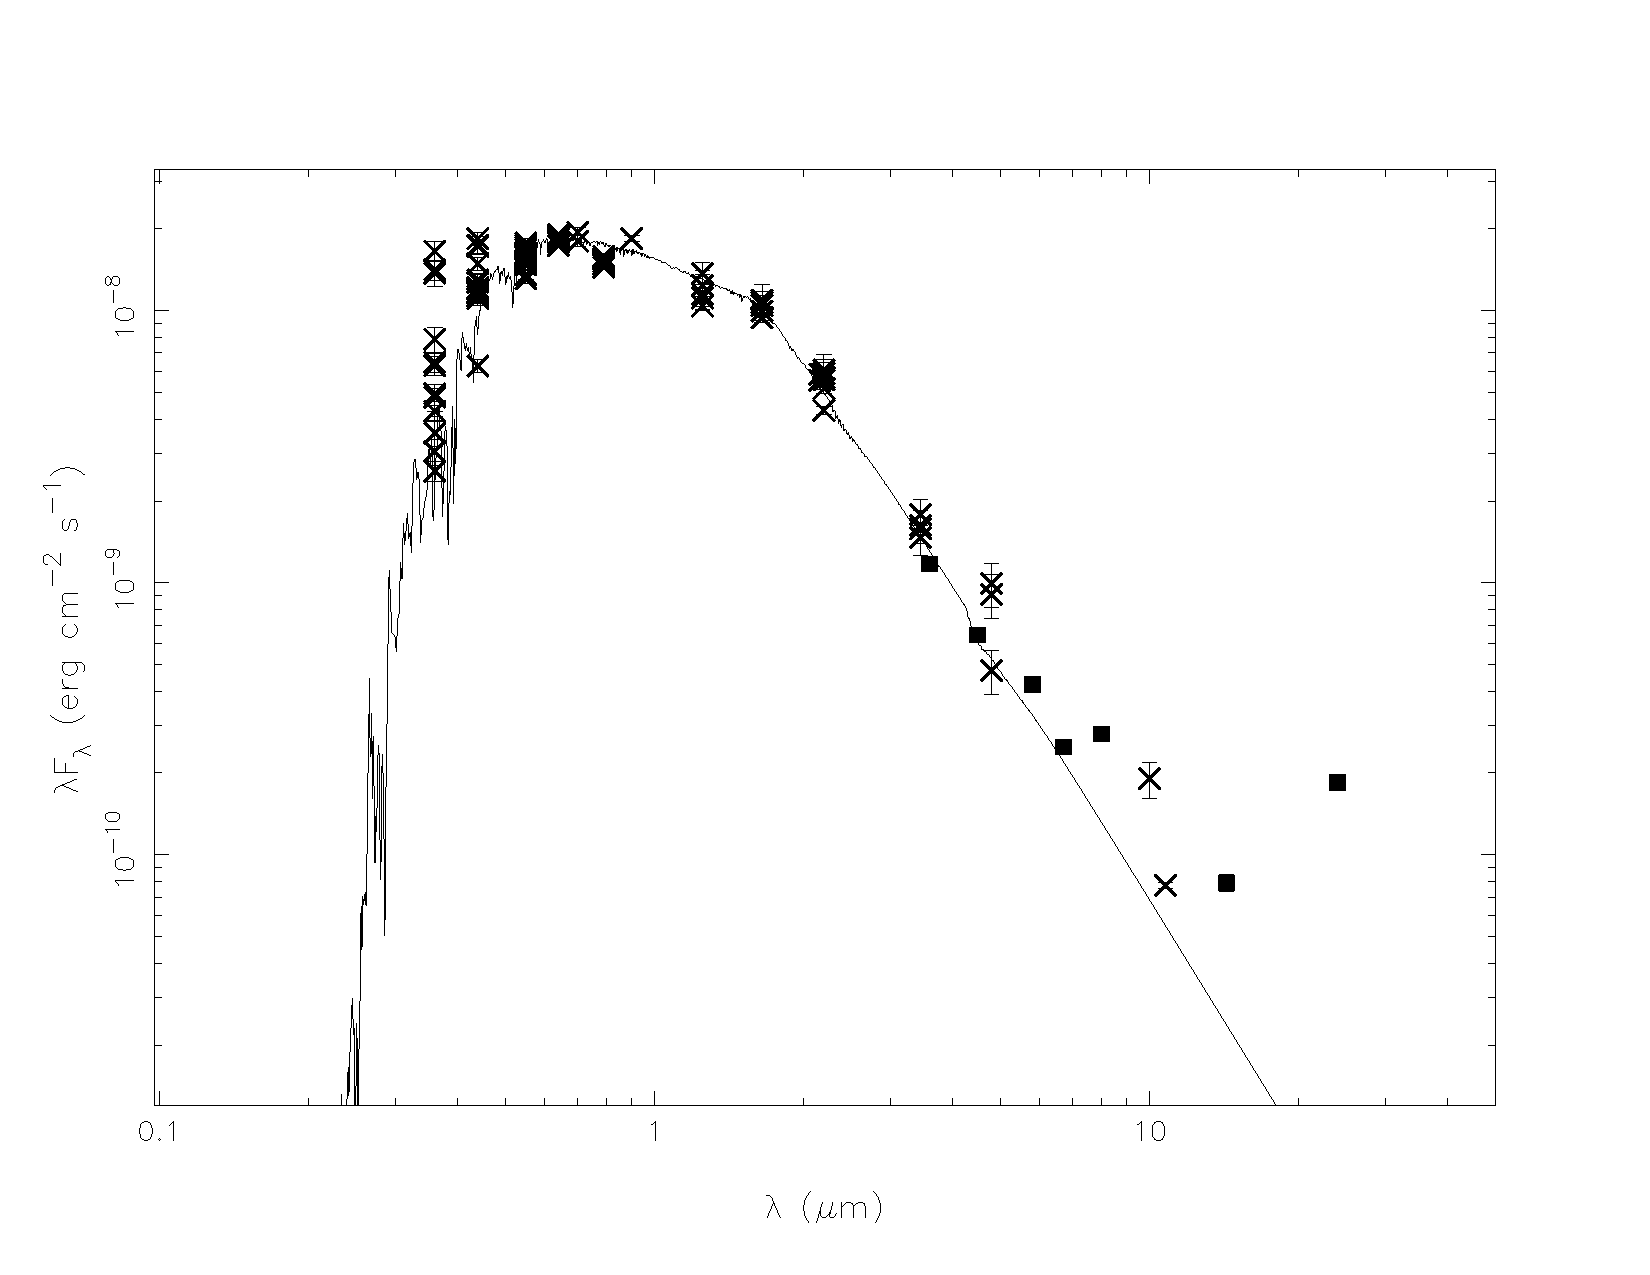
\includegraphics[angle=0,scale=0.30]{doar21_sed.pdf}
% Give the caption for the Figure here. 
\caption{Example figure: The spectral energy distribution of DoAr 21,
  from ultraviolet (4000 \AA) through infrared wavelengths. Spitzer and ISO data
  are shown as filled squares, and the 850 \micron\ and 1.3 mm
  upper limits are not shown.  The photometry has been de-reddened
  with $A_V = 6.2$ and $R_V = 4.2$ as described in the text.
  Overplotted is a model photosphere (solid line); the star shows a
  clear infrared excess at $\lambda \ge 8$ \micron.}
% This label can be used in the text to refer to the figure by number, if
% desired; see example \ref command in the text where this figure is
% referred to. 
\label{figure:sed}
\end{figure}


% Here's an example table, using the AASTeX \deluxetable
% environment.  If you don't need the fancy features of \deluxetable,
% you can just use \table or \tabular.  I haven't tested it
% extensively, but it seems like using \deluxetable makes it a little
% harder to squeeze tables into a smaller amount of space (and gives
% you a little less control over their placement) than the regular
% \table environment. 

\begin{deluxetable}{lccc}
\centering
% This sets the table to its 'natural' width, i.e. not trying to
% expand to the width of the text:
\tablewidth{0pt}  
\tablecaption{Example table: Photometry of DoAr 21\label{table:gemini-photometry}
}
\tablehead{
  \colhead{Filter} & \colhead{Flux within  0\farcs82} &
 \colhead{Flux within 2\farcs75} &  \colhead{Flux within 6\arcsec}\\
\colhead{} & \colhead{(mJy)} &\colhead{(mJy)}&\colhead{(mJy)}}
\startdata
\phn 8.6 \micron\ (PAH)  & 313  & 525  & 596 \\
10.4 \micron\  (Si-4)      & 176  & 300  & 347 \\
11.3 \micron\ (PAH) & 234  & 680  & 816 \\
%18.3 \micron\ (Qa)       & 165  & 607  & 728 \\
\enddata
\end{deluxetable}

\section{Observations and/or Theory}

Observations could go here (Table \ref{table:gemini-photometry}), and
so on.  We might also want to include figures in your paper (Figure
\ref{figure:sed}).   Note that the symposium proceedings are printed in
black and white, so you should either convert your figures to
grayscale, or at minimum ensure that they are still legible when
printed that way.

Or perhaps your work is more theoretical, and has some mathematical
notation embedded in it.  It's easy to display math in-line (e.g.\ the 
code  \verb|$L = 4 \pi R_*^2 \sigma T^4$| produces $L = 4
\pi R_*^2 \sigma T^4$) or to have equations that are separated from
the rest of the text, either using \$\$ or  \verb|\begin{equation}|
and  \verb|\end{equation}|  commands to surround them: 

\begin{equation}
F_\nu = \frac{L_\nu}{4\pi d^2}
\end{equation}




\section{Length Guidelines}

You should aim for a five-page paper (or eight pages if you are
co-authoring a paper with multiple students).  However, one of the
slightly tricky things about \LaTeX\ is that you don't have much
control over where it places figures and tables. (If you look at the
source for this file, you may find that the figure and table don't
come out in the document exactly where the code to produce them was
located.  They will never come out {\em earlier} in the text, but they
will often come out later.)  If you find that \LaTeX\ is (perhaps
inexplicably) pushing your paper to six pages because it insists on
putting a table or figure onto a different page, or leaves some blank
space on a page, you can try playing around with where in the text you
insert the commands to produce the figure or table.  Ultimately, if
you have a hard time getting it work, don't drive yourself (or your
advisor) crazy trying to fiddle with it.

\section{Getting Help}

See the \LaTeX\ source code for this example document to get a sense
of how particular commands produce the output you see here.  The
source document also has extensive comments explaining what the
structure of the document is, and how particular commands work. 

There are many print and on-line resources for help with \LaTeX.  See
the AAS web page \url{http://aas.org/aastex/aastex-documentation} for
help with commands specific to AASTeX.  In particular, there is a list
of AASTeX symbols, including favorites like \verb|\sun| ($\sun$) and
the Angstrom symbol \verb|\AA| (\AA), at
\url{http://authortools.aas.org/aastex/aassymbols.pdf}.

For citing references in the text and in the bibliography, most of
this will take care of itself automatically if you copy your
bibliographic entries from NASA ADS (see below) and cite them in the text using \verb|\citet| or \verb|\citep| as outlined above. You can either use this method where you copy the \verb|\bibitem| entries directly into this \verb|main.tex| file, however some of you may like to use Bibtex - in which case comment out the \verb|%\bibitem| lines (with the \% sign) and instead copy the full Bibtex code into the \verb|references.bib| file. Discuss the preferred method with your supervisor. If you have any
additional questions (e.g., how to cite something not listed in ADS,
follow the guidelines given for the {\it Astrophysical Journal}\/ at
\url{http://aas.org/authors/manuscript-preparation-aj-apj-author-instructions}. 
  
% Give the acknowledgments here.  Citing the NSF grant that funds the
% REU program is a good idea (just using the text below).  In the
% interest of saving space, there is no section heading inserted here
% specifically for acknowledgments. 

\acknowledgments

Here is where you thank people (and funding agencies!)  There is no
explicit section header in the output; just make this the last thing
before the bibliography, preceded by the \verb|\acknowledgments| 
command. For example:  We gratefully acknowledge support from KNAC Funding, or local funding sources. This research has
made use of the SIMBAD database, operated at CDS, Strasbourg, France, and of NASA's Astrophysics Data System. 



% Here's how we specify the bibliography. 

\begin{thebibliography}{}
% For including references in the final reference list, you can get
% Latex-formatted references directly from NASA ADS
% (https://ui.adsabs.harvard.edu/) - after
% finding the reference you want, click on "Export Citation" in the left menu. 
% You want the AASTex version which will look something like this: 
% \bibitem[Salyk et al.(2019)]{2019ApJ...874...24S} Salyk, C., Lacy, J., Richter, M., et al.\ 2019, \apj, 874, 24
% This can be pasted in your document. 
% This method is tedious and prone to error if you have lots of references (see comments below on using Bibtext instead.)

% Note that each \bibitem record has three parts: the first part in
% curly braces is how the citation will appear in the text; the second
% is a shorthand tag that you use to refer to the paper by name; and
% the third is the contents of the bibliography entry.  Leave the
% first and third parts alone, but you can edit the second part (in
% square braces) to be whatever abbreviation you want to use to refer
% to that paper - here I've changed the default ones that come from
% ADS to be something I can remember more easily (usually just an
% author and year).  These are the tags that are used above in the
% \citet and \citep commands. 

\bibitem[Bary et al.(2002)]{Bary2002} Bary, J.~S., Weintraub, D.~A., \& Kastner, J.~H.\ 2002,  \apjl, 576, L73 
\bibitem[Kwitter et al.(2013)]{Kwitter2013} Kwitter, K.~B., Lehman,  E.~M.~M., Balick, B., \& Henry, R.~B.~C.\ 2013, \apj, 768, 97 
\bibitem[Willman \& Strader(2012)]{Willman2012} Willman, B., \& Strader, J.\ 2012, \aj, 144, 76 
\end{thebibliography}

%If you prefer to use Bibtex uncomment the below two lines, and comment out (with % sign) the \bibitem lines above (from and including both \begin{thebibliography}{} and \end{thebibliography}
%%%% Look how much neater it is in Bibtex, and note that there is an entry in the references.bib which is not mentioned in the text, and therefore not listed in the references. 
%You can get the things you need to put into the .bib to make this work either from ADS (under the Export Citation tab) or through a citation manager like Zotero. 
%
%\bibliographystyle{mnras}
%\bibliography{references.bib} % if your bibtex file is called references.bib

\end{document}
